\chapter{A2: RetinaNet và Faster R-CNN trên VOC2012}
\label{chap:a2}
\section{Bài toán và dữ liệu}
Khác với phân loại ở A1, mỗi ảnh ở A2 có thể chứa nhiều đối tượng thuộc nhiều
lớp. Mạng phải đồng thời dự đoán nhãn, bounding box và độ tin cậy.
Thí nghiệm so sánh RetinaNet một giai đoạn với Faster R-CNN hai giai đoạn.
Cả hai dùng ResNet-50 pretrained ImageNet và FPN; sự khác biệt nằm ở các mức
pyramid, anchors, cách chọn mẫu và detection head.

PASCAL VOC2012 \cite{voc,vocdevkit} có 20 lớp và 11.540 ảnh trainval có nhãn.
Toàn bộ số ảnh này được chia 80/10/10 bằng seed 42; các tập không giao nhau
theo định danh ảnh. Test trong báo cáo là \emph{holdout nội bộ}, không phải
test chính thức VOC2012; không so trực tiếp với leaderboard của cuộc thi.
Manifest tham chiếu JPEG/XML có sẵn, không nhân bản ảnh.
Việc sử dụng tuân theo VOC Database Rights; quyền đối với từng ảnh thuộc
về tác giả/chủ sở hữu gốc. Nguồn tải và định dạng nhãn được ghi trong README dữ liệu.
\DataTable{assets/a2/dataset.tex}{Số ảnh và annotation VOC2012. Một bbox có thể vừa difficult vừa truncated.}
Nhãn XML gồm tên lớp, \texttt{bndbox}, \texttt{difficult} và \texttt{truncated}.
Tọa độ VOC đánh số từ 1, bao gồm cả hai đầu, được chuyển thành khoảng nửa mở
đánh số từ 0: $[x_{\min}-1,y_{\min}-1,x_{\max},y_{\max}]$.
Dataset trả về tensor RGB và danh sách bbox, class ID 1--20 cùng các cờ annotation.
RetinaNet ánh xạ nhãn sang 0--19 khi tính loss, rồi chuyển về 1--20 khi suy luận.
Faster R-CNN dành ID 0 cho background.

\ReportFigure{assets/a2/class_distribution.png}{Phân bố bbox thường của 20 lớp trong train, validation và test; mỗi panel dùng trục riêng.}
Person chiếm 6.802/21.975 bbox thường ở train, khoảng 30,95\%; sofa chỉ có
447 bbox. Báo cáo dùng cả AP từng lớp và macro-F1 để nhìn ảnh hưởng của
mất cân bằng. Tổng theo lớp là số đối tượng, không phải số ảnh.
\ReportFigure{assets/a2/bbox_distribution.png}{Kích thước, tỷ lệ cạnh bbox và chiều rộng/cao ảnh gốc.}
BBox đa dạng về scale và tỷ lệ cạnh. FPN cung cấp nhiều stride, còn ba
aspect ratio bao phủ vật thể cao, vuông và rộng.

\section{Tiền xử lý và DataLoader}
Resize giữ tỷ lệ, cạnh ngắn 600 px, cạnh dài tối đa 1.000 px. Phóng ảnh
không bổ sung chi tiết đã mất ở ảnh gốc. Tensor nằm trong $[0,1]$; model
chuẩn hóa ImageNet một lần. Batch được pad đến bội số 32, nên VRAM
còn phụ thuộc tỷ lệ cạnh các ảnh cùng batch. Không chia tiles.

Train áp dụng horizontal flip xác suất 0,5 và biến đổi bbox tương ứng;
validation/test không có augmentation. DataLoader shuffle train, workers 0,
không bỏ batch cuối. Cả hai mạng học toàn bộ bbox có nhãn, kể cả
difficult. Khi đánh giá, difficult không tính vào số GT thường và detection
khớp difficult được bỏ qua theo VOC. Truncated vẫn được học/đánh giá.
\ReportFigure{assets/a2/preprocessing.png}{Ảnh gốc, resize giữ tỷ lệ và horizontal flip; bbox đi cùng phép biến đổi.}

\section{FPN: phương pháp, thí nghiệm và giới hạn}
Feature tầng sớm giữ chi tiết vị trí, trong khi tầng sâu có ngữ nghĩa mạnh
hơn. FPN \cite{fpn} kết hợp chúng bằng top-down và lateral connections.
ResNet-50 xuất C2--C5, strides 4/8/16/32, channels 256/512/1.024/2.048.
Với lateral $L_l$ là Conv $1\times1$ đưa về 256 channels:
\begin{equation}
T_5=L_5(C_5),\quad
T_l=L_l(C_l)+\operatorname{Upsample}_{\mathrm{nearest}}(T_{l+1}),\quad
P_l=\operatorname{Conv}_{3\times3}(T_l).
\end{equation}
Upsample đến đúng shape lateral; nhánh top-down truyền $T$ trước smoothing,
không truyền $P$ sau smoothing. Neck không thêm BN/ReLU tại các mức này.

\begin{table}[H]\centering\caption{Kết quả và ablation của FPN trên COCO; số liệu tác giả \cite{fpn}.}
\small\begin{tabularx}{\linewidth}{Xrr}\toprule
Thiết lập & Chỉ số & Giá trị\\\midrule
Table 1, ResNet-50 RPN C4 & AR@1k &48,3\\
RPN FPN đầy đủ & AR@1k &56,3\\
Bỏ top-down / bỏ lateral & AR@1k &49,5 / 46,1\\
Chỉ P2, tăng anchors lên 750k & AR@1k &51,3\\
Table 3, Faster R-CNN C4 / FPN & AP &31,6 / 33,9\\
Table 3, Faster R-CNN C4 / FPN & AP50 &53,1 / 56,9\\\bottomrule
\end{tabularx}\end{table}
Paper dùng COCO trainval35k và minival 5 k cho ablation. Bỏ một nhánh làm
giảm recall; chỉ tăng số anchors ở P2 chưa đạt FPN đầy đủ. Kết quả hỗ trợ
vai trò phối hợp ngữ nghĩa và độ phân giải, ngoài việc tăng số vị trí dự đoán.
Thí nghiệm VOC dùng FPN cho cả hai mạng; không có ablation bỏ nhánh để đo
riêng đóng góp của neck. FPN tăng activation ở mức độ phân giải cao và
không tự giải quyết vật thể quá nhỏ, che khuất hoặc nhãn nhiễu.

\section{RetinaNet và Focal Loss}
\subsection{Động cơ và hàm mất mát}
Các anchors phủ dày trên ảnh tạo nhiều mẫu nền dễ phân loại, có thể lấn át
gradient từ đối tượng thật. Focal Loss \cite{retina} giảm đóng góp của mẫu đã được dự đoán đúng:
\begin{equation}
\operatorname{FL}(p_t)=-\alpha_t(1-p_t)^\gamma\log p_t,\qquad
\alpha=0,25,\quad\gamma=2.
\end{equation}
Với $p_t=0,9$, hệ số điều chỉnh là 0,01; với $p_t=0,1$ là 0,81.
$\alpha_t=\alpha$ cho mẫu dương, $1-\alpha$ cho mẫu âm; đây là cân bằng
foreground/background, không phải cân bằng tần suất 20 lớp.
Mỗi anchor có 20 xác suất sigmoid độc lập, không thêm một logit background.
Loss phân loại chuẩn hóa theo số anchors dương; bbox dùng Smooth L1
beta 1. Bias classification khởi tạo theo xác suất tiên nghiệm của foreground $\pi=0,01$.

\begin{table}[H]\centering\caption{RetinaNet Table 1: ablation trên COCO minival và đánh đổi tốc độ/AP trên test-dev; số liệu tác giả \cite{retina}.}
\small\begin{tabularx}{\linewidth}{Xrr}\toprule
Thiết lập & AP & Thời gian\\\midrule
\multicolumn{3}{l}{Ablation, COCO minival (Table 1a--d)}\\
Alpha-balanced CE tốt nhất / Focal Loss &31,1 / 34,0&--\\
3 scales $\times$ 3 ratios &34,0&--\\
ResNet-101: OHEM tốt nhất / Focal Loss &32,8 / 36,0&--\\
\multicolumn{3}{l}{Tốc độ/chất lượng, COCO test-dev (Table 1e)}\\
ResNet-50, cạnh ngắn 500 &32,5&72 ms\\
ResNet-50, cạnh ngắn 800 &35,7&153 ms\\\bottomrule
\end{tabularx}\end{table}
Paper dùng COCO trainval35k; thời gian đo trên GPU M40. Focal Loss cải thiện
2,9 điểm AP so với CE được cân bằng; trên ResNet-101, hơn OHEM tốt nhất
3,2 điểm AP. Tăng resize cũng tăng AP nhưng tốn
thời gian. Các kết quả giải thích lựa chọn loss/scale, không phải mốc trực
tiếp cho holdout VOC. Mẫu khó cũng có thể là annotation nhiễu; tập trung
vào chúng không bảo đảm giải quyết mọi lớp hiếm hoặc che khuất.

\subsection{Neck, anchors và head}
RetinaNet dùng P3--P7. P3--P5 lấy từ C3--C5; P6 là Conv $3^2$/stride 2
trên C5; P7 là Conv $3^2$/stride 2 trên ReLU(P6).
\begin{figure}[H]\centering
\resizebox{.83\linewidth}{!}{\ArchFPN{1}}
\caption{FPN RetinaNet. Shape minh họa tại input $512\times512$; thí nghiệm dùng resize 600/max 1000. Độ sâu khối thể hiện channels, không dùng cùng tỷ lệ với kích thước không gian.}
\end{figure}
Anchor bases 32/64/128/256/512, scales $1,2^{1/3},2^{2/3}$, ratios
$0,5,1,2$ tạo 9 anchors/vị trí. IoU $\geq0,5$ là positive, $<0,4$ là
negative, khoảng giữa bỏ qua; matching giữ low-quality matches theo torchvision.
Hai subnet có trọng số riêng; mỗi subnet gồm bốn Conv $3^2$/256 + ReLU
và một Conv output. Trọng số mỗi subnet dùng chung trên các mức.
\begin{figure}[H]\centering
\resizebox{.98\linewidth}{!}{\ArchRetinaHead}
\caption{RetinaNet head: $9\times20=180$ class logits, $9\times4=36$ offsets mỗi vị trí; không có logit background riêng.}
\end{figure}

\section{Faster R-CNN: RPN và RoI head}
Faster R-CNN \cite{faster} tạo đề xuất vùng rồi phân loại/hiệu chỉnh vùng.
FPN dùng P2--P6 cho RPN; P6 là MaxPool $1^2$/stride 2 trên P5.
RoI head dùng P2--P5.
\begin{figure}[H]\centering
\resizebox{.83\linewidth}{!}{\ArchFPN{2}}
\caption{FPN Faster R-CNN: P2 có độ phân giải cao, P6 lấy từ P5. Shape ở input $512\times512$ chỉ để đối chiếu cấu trúc.}
\end{figure}
RPN gồm Conv $3^2$/256 + ReLU và hai nhánh $1^2$ cho objectness/bbox.
Bases 32--512, một scale, ba ratios tạo 3 anchors/vị trí.
Positive IoU $\geq0,7$ hoặc best anchor, negative $<0,3$; sample
256 anchors/ảnh, tối đa 50\% positive. NMS proposals dùng 0,7,
giữ 2.000 proposals/train và 1.000/test.

RoI gán mức theo FPN:
\begin{equation}
k=\operatorname{clip}_{[2,5]}
\left\lfloor4+\log_2\left(\frac{\sqrt{wh}}{224}\right)\right\rfloor.
\end{equation}
RoI Pooling $7^2$ lượng tử hóa tọa độ và max pooling, không dùng RoIAlign.
Tensor $7\times7\times256$ flatten thành 12.544, qua hai FC 1.024 + ReLU
rồi tách 21 logits và 84 class-specific offsets. Train sample 512 RoIs/ảnh,
tối đa 25\% positive. Bốn loss gồm RPN objectness/bbox và RoI classification/bbox;
hai bbox loss dùng Smooth L1 beta $1/9$.
\begin{figure}[H]\centering
\resizebox{.98\linewidth}{!}{\ArchFasterHead}
\caption{Faster R-CNN: RPN tạo proposals, RoI Pool gom feature, hai FC trước hai nhánh output.}
\end{figure}
Hai mạng cùng decode bbox, score floor 0,05, class-wise Hard-NMS 0,5,
cap 100 detections/ảnh. RetinaNet lọc top 1.000 candidates/mức trước NMS.
Gallery dùng score từ 0,30 và tối đa 15 boxes; metric không bị giới hạn
theo số box hiển thị.
\DataTable{assets/a2/capacity.tex}{Số tham số trainable. FrozenBatchNorm giữ statistics/buffers cố định.}

\section{Huấn luyện và lựa chọn weights}
ResNet-50 nạp ImageNet-1K V1, bỏ FC ImageNet; các Conv được fine-tune.
Các lateral/smoothing chung khởi tạo giống nhau theo seed; head và neck
bổ sung khởi tạo mới. Không nạp pretrained detection trên COCO.

SGD LR 0,01, momentum 0,9, weight decay $10^{-4}$; warmup một epoch từ
0,1 lần LR rồi cosine đến 0,01 lần LR. Clip gradient norm 10, AMP
float16 cho convolution; RetinaNet loss/RoI Pool tính FP32.
Batch train/eval 4, accumulation 3, effective batch 12.
Mỗi epoch có 2.308 batches train, 289 validation; test cũng có 289.
Gradient chuẩn hóa theo số ảnh thực của cửa sổ, kể cả cửa sổ cuối.

Giới hạn 30 epoch; dừng sớm theo validation VOC mAP50, patience 2,
min-delta 0,001. Chỉ cập nhật checkpoint khi vượt best đang giữ hơn
min-delta. Best weights theo quy tắc này giữ trong CPU RAM.
Hai lượt train/validation hoàn tất trước khi mở test; test không chọn
epoch hoặc confidence.
\DataTable{assets/a2/training.tex}{Epoch thực chạy, epoch chọn, validation mAP50 và số cập nhật SGD.}
RetinaNet dừng ở epoch 23, dùng epoch 21; Faster R-CNN dừng ở epoch 13,
dùng epoch 11. Tổng 36 epoch, 27.720 cập nhật, không AMP skips.
Train + validation lần lượt 8 giờ 01 phút 47 giây và 4 giờ 57 phút
25 giây, gồm tải dữ liệu và tính metric, không gồm test/vẽ hình.

\subsection{Phạm vi đối chiếu paper}
FPN paper dùng COCO và feature sharing bốn bước; cài đặt VOC train joint
RPN/RoI. RetinaNet paper dùng batch 16/lịch 90k iterations với các mốc giảm LR;
ở đây dùng epoch/cosine/dừng sớm. Resize chung 600/max 1000, ResNet-v1.5,
anchor rounding, low-quality matching và Smooth L1 theo torchvision cũng
khác một số chi tiết của tác giả. Thí nghiệm sử dụng nguyên lý neck/head của paper; các khác biệt trên giới hạn
khả năng đối chiếu trực tiếp với kết quả COCO của tác giả.

\section{Chỉ số đánh giá}
VOC2010--2012 mAP50 all-point là metric chính: sort score, matching
one-to-one cùng class, IoU $>0,5$, tích phân precision envelope theo recall
\cite{vocdevkit}. Duplicate thường là FP; matches difficult bị bỏ qua.
VOC07 AP11 bổ sung để phân biệt cách nội suy.

COCO-style AP trung bình 10 ngưỡng IoU 0,50--0,95, bước 0,05, 101 recall
points, max 100 detections/ảnh \cite{cocometrics}. AP50/AP75 và AP/AR theo
scale bổ sung phân tích định vị. Small/medium/large dùng diện tích bbox ảnh
gốc, theo mốc $32^2/96^2$. Evaluator giữ union IoU và bỏ qua repeated
matches difficult theo VOC. Đây là metric COCO-style trên VOC, không phải
dataset COCO. VOC AP50 và COCO-style AP50 khác cách nội suy/biên IoU.

P/R/F1 dùng matching class-wise VOC tại score 0,30; micro-F1 gộp TP/FP/FN,
macro-F1 trung bình 20 lớp. Ma trận chẩn đoán dùng class-agnostic greedy
theo score, IoU $\geq0,5$, để nhìn nhầm lớp. Background biểu diễn FP/FN.
Matched IoU là trung bình TP trong chẩn đoán, không thay thế AP.
Score floor/cap chung có thể giới hạn recall, được giữ như nhau ở hai mạng.

\section{Kết quả test và so sánh}
\DataTable{assets/a2/results.tex}{Test holdout 1.154 ảnh, 2.687 bbox thường. Metric ở thang 0--1.}
Faster R-CNN đạt VOC mAP50 0,7307, hơn RetinaNet 1,49 điểm phần trăm.
COCO-style AP50:95 đảo thứ tự: RetinaNet 0,4136 so với 0,4075, hơn 0,61 điểm.
AP75 riêng lẻ vẫn cao hơn ở Faster R-CNN (0,4245 so với 0,4149).
Vì vậy không dùng một ngưỡng IoU để khẳng định toàn bộ chất lượng định vị.
Validation mAP50 cao hơn test 3,43 điểm ở RetinaNet, 2,29 điểm ở Faster R-CNN.

Tại score 0,30, Faster R-CNN recall cao hơn (0,8269 so với 0,7983),
nhưng precision thấp hơn (0,4053 so với 0,4625). RetinaNet có micro-F1
cao hơn (0,5857 so với 0,5440). Đánh đổi precision--recall ở một confidence cố định không
mâu thuẫn với thứ tự mAP50, vì AP tổng hợp cả đường precision--recall.
Ngưỡng confidence được giữ cố định khi đánh giá test.
\DataTable{assets/a2/scale_recall.tex}{COCO-style AP theo scale và AR trung bình qua các ngưỡng IoU.}
APsmall thấp ở cả hai: 0,1057/0,1487, trong khi APlarge là 0,4687/0,4645.
Faster R-CNN hơn APsmall 4,30 điểm, song còn khác anchors/head/sampling,
chưa thể quy toàn bộ lợi ích cho P2. AR@10 gần AR@100: tăng detections
giữ lại từ 10 lên 100 chỉ cải thiện recall trung bình ít trong thiết lập này.
\ReportFigure{assets/a2/learning_curves.png}{Loss train và validation VOC mAP50/COCO-style AP; nét đứt đứng chỉ epoch được chọn.}
Loss train tiếp tục giảm khi validation gần bão hòa. RetinaNet học nhiều
epoch hơn nhưng không vượt Faster R-CNN ở mAP50 test. Độ lớn tổng loss
không dùng xếp hạng hai kiến trúc vì thành phần/chuẩn hóa khác nhau.
\ReportFigure{assets/a2/loss_components.png}{Hai thành phần loss RetinaNet và bốn thành phần RPN/RoI; mỗi panel có trục riêng.}

\subsection{Chi phí huấn luyện và suy luận}
\DataTable{assets/a2/cost.tex}{Chi phí trên RTX A3000 12 GB Laptop; peak là allocated PyTorch, không phải tổng VRAM.}
RetinaNet có 36,67 triệu tham số, ít hơn Faster R-CNN 4,73 triệu.
Train + validation trung bình mỗi epoch khoảng 20,95/22,88 phút.
Faster R-CNN chạy ít epoch nên thời gian tổng thấp hơn 184,37 phút.
Số tham số và số giai đoạn chưa đủ để dự đoán chi phí huấn luyện tổng.

Benchmark CUDA events warmup ba lượt; batch 1 đo 20 lần, batch 4 đo 10 lần.
Latency model gồm resize, normalize, backbone, neck, head, decode/NMS;
không gồm đọc JPEG/metric CPU. Median batch 1 là 47,35/48,92 ms,
tương ứng 21,12/20,44 FPS; RetinaNet nhanh hơn khoảng 3,3\% theo FPS.
Throughput batch 4 thấp hơn FPS batch 1. Các batch dùng ảnh khác tỷ lệ
cạnh/padding nên không đọc hai cột như phép đo scaling với workload
đồng nhất. Pipeline test gồm đọc ảnh, chuyển tensor và thu predictions,
đạt 17,00/16,31 ảnh/s.
\ReportFigure{assets/a2/comparison.png}{So sánh AP, latency batch 1 và peak allocated VRAM; số và đơn vị ghi trên đồ thị.}

\section{Theo lớp, ma trận và trường hợp sai}
\DataTable{assets/a2/per_class.tex}{R=RetinaNet, F=Faster R-CNN; AP là COCO-style AP50:95, F1 tại score 0,30.}
Cat, bus và dog có AP50 cao; pottedplant/chair thấp ở cả hai.
Faster R-CNN cải thiện diningtable từ 0,3852 lên 0,6225, nhưng RetinaNet
cao hơn ở horse (0,8309/0,7675) và aeroplane (0,8042/0,7523).
Các chỉ số trung bình che khuất một phần chênh lệch giữa các lớp.
\ReportFigure{assets/a2/per_class_ap.png}{VOC AP50 và COCO-style AP theo lớp; hai detector dùng chung mỗi panel.}
Ma trận ở Phụ lục trình bày riêng số đếm và tỷ lệ theo hàng. Hàng background là detection
không ghép GT; cột background là GT bị bỏ sót. Lệch bbox, dự đoán lặp và
nhầm lớp đều có thể tạo FP/FN. P/R/F1 chính được tính class-wise riêng,
không lấy trực tiếp từ ma trận chẩn đoán.

Ba ảnh lỗi minh họa chủ yếu là dự đoán thừa: mỗi ảnh có một TP và không
có FN theo chẩn đoán tại score 0,30. Ở ảnh con chó giữa các chân người,
RetinaNet/Faster R-CNN có 8/9 FP; nhiều bbox lặp hoặc chỉ bao phủ một phần
vật thể. Ảnh xe đồ chơi có 10/5 FP, với các dự đoán chair/car không khớp
annotation. Ảnh trang trí nội thất có 10/8 FP, gồm nhiều bbox pottedplant/chair.
Những hình này cho thấy sự khác nhau giữa một vùng trông giống đối tượng
và một detection khớp nhãn theo IoU. Chúng không đại diện cho tỷ lệ lỗi
toàn tập; số đếm đầy đủ nằm trong ma trận và metric test.

\section{Kết luận A2 và giới hạn}
Faster R-CNN có lợi thế mAP50, recall và APsmall; RetinaNet có lợi thế
COCO-style AP tổng hợp, F1 tại score 0,30, số tham số và latency batch 1.
Nếu ưu tiên recall vật thể nhỏ, Faster R-CNN phù hợp hơn theo số liệu này;
nếu cân bằng AP nhiều ngưỡng IoU và chi phí suy luận, RetinaNet đáng cân nhắc.

Kết luận dựa trên một seed và holdout nội bộ. Hai mạng khác nhiều thành
phần cùng lúc, chưa cô lập riêng P2, Focal Loss hoặc proposals. Giới hạn
epoch/dừng sớm, score floor/cap và resize chung ảnh hưởng phép so sánh.
Các hướng tiếp theo là nhiều seed, ablation neck/anchors với head giữ cố
định và chọn confidence bằng validation; chưa nằm trong kết quả báo cáo.

\begin{landscape}\begin{figure}[p]\centering
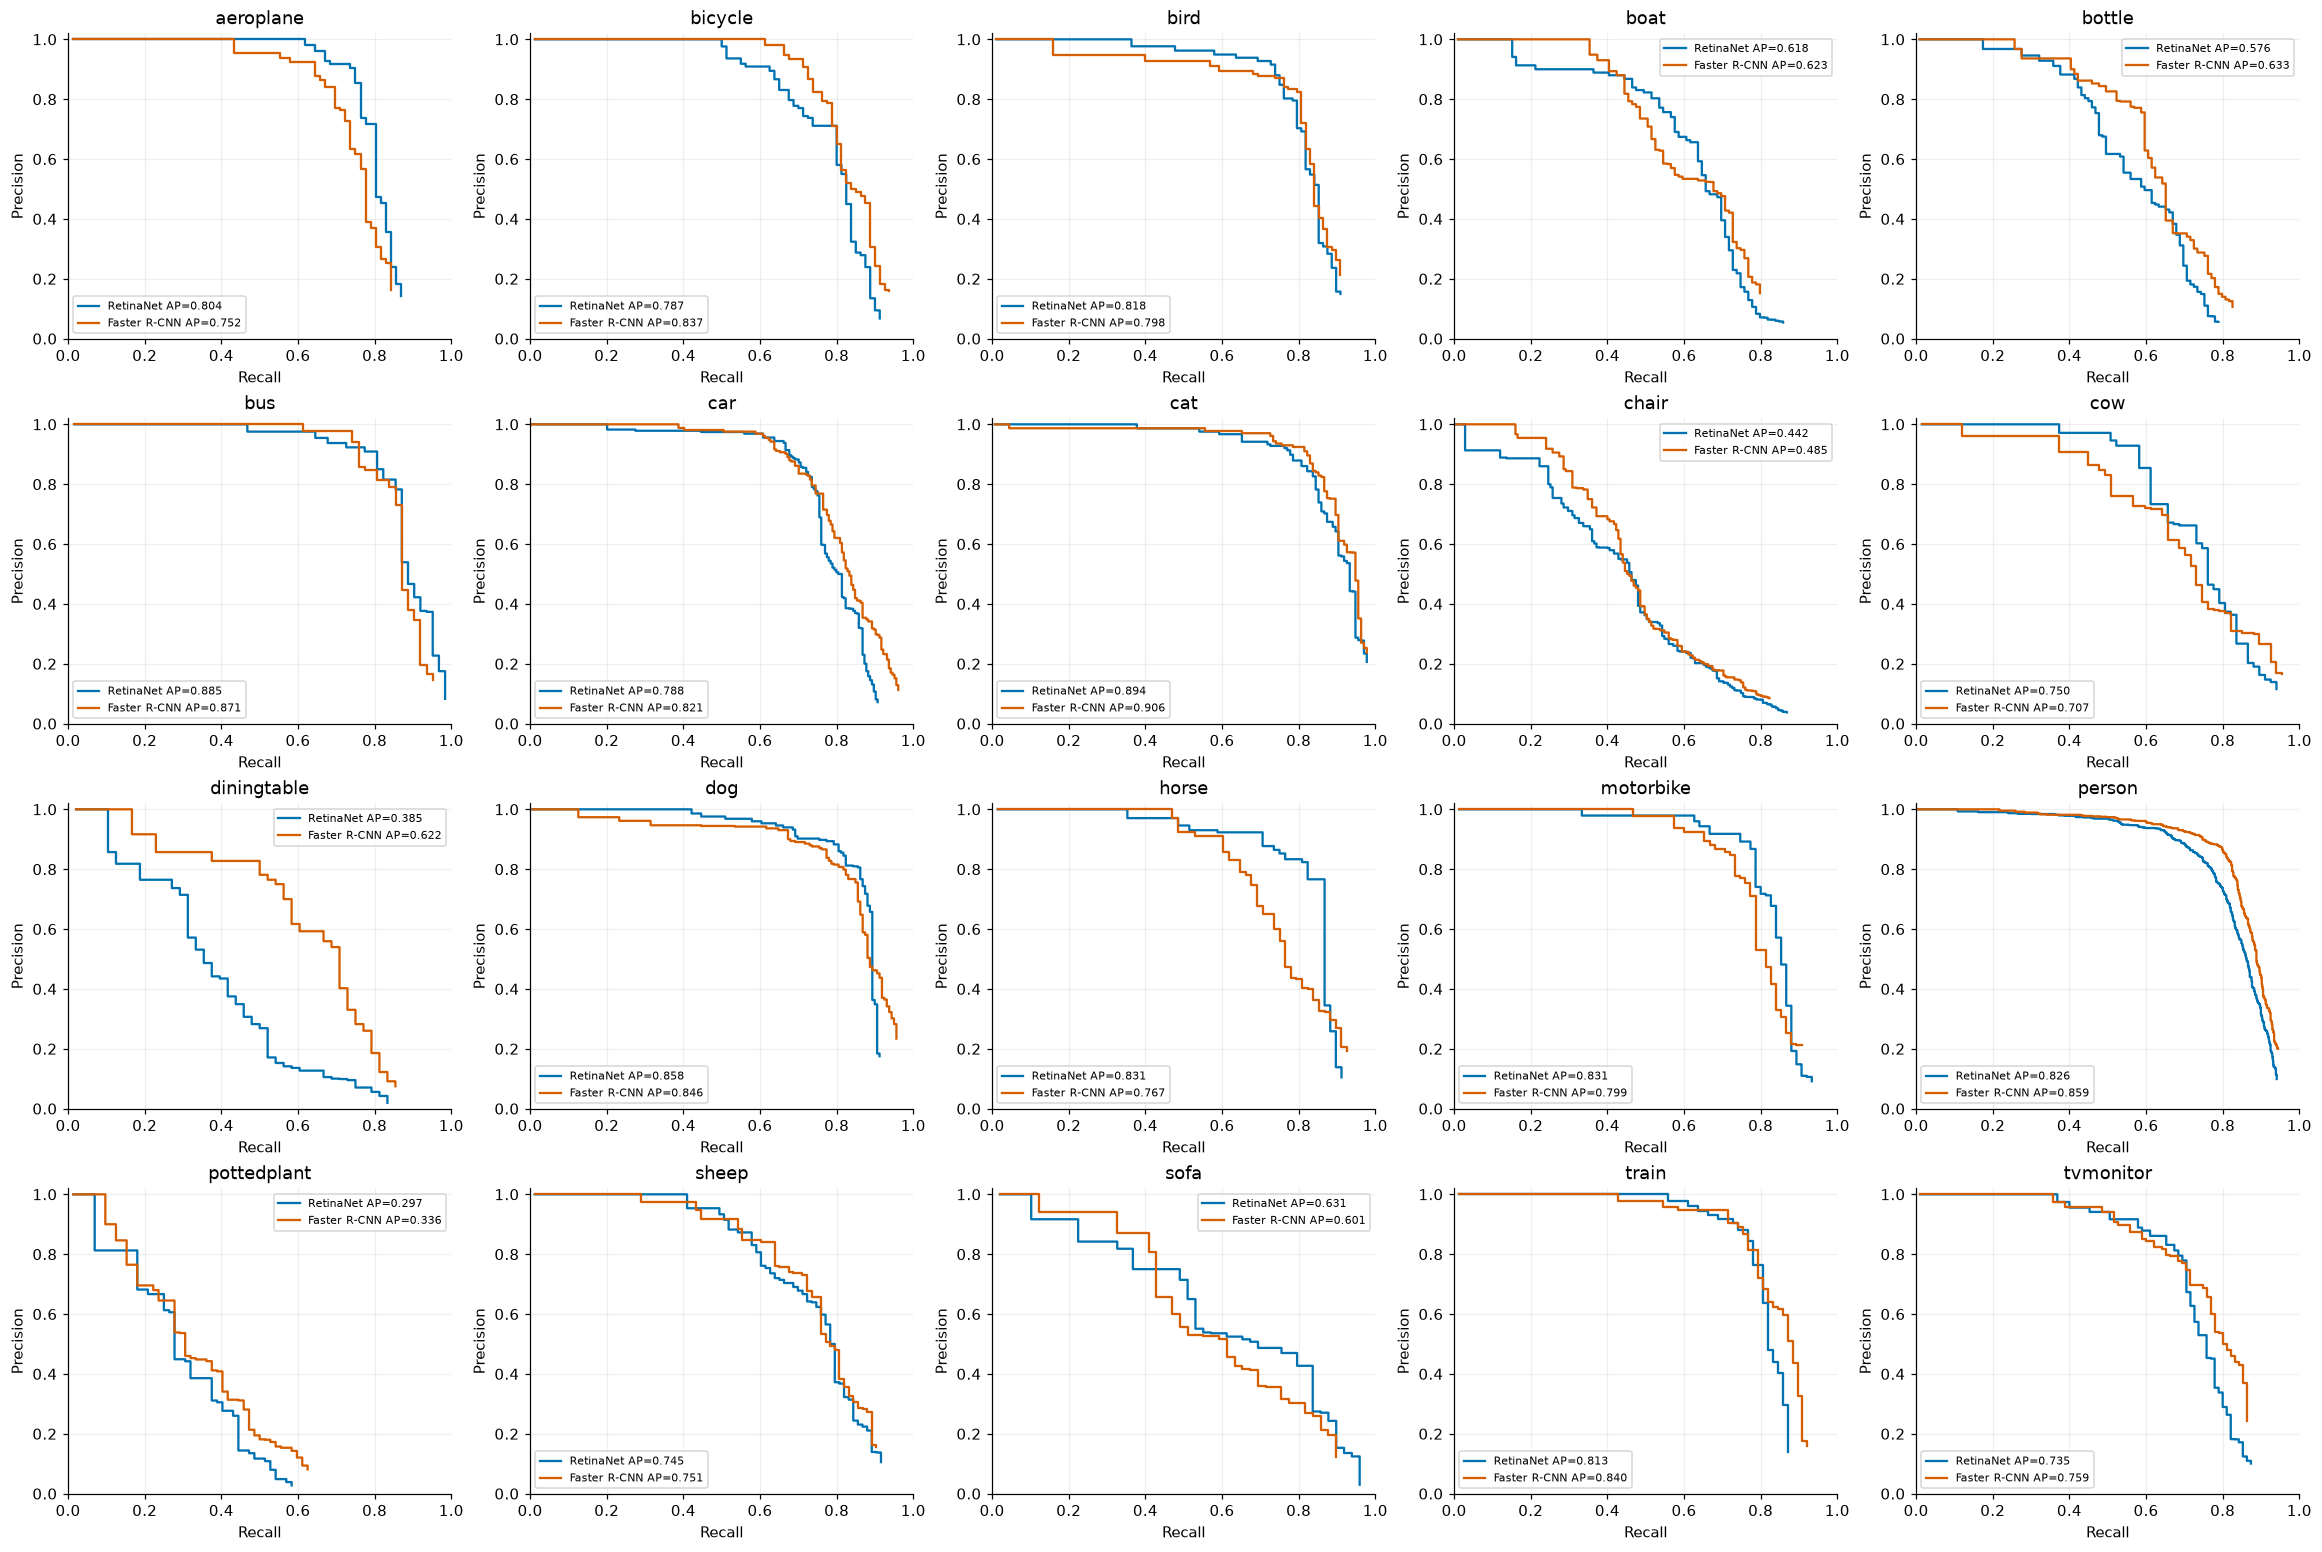
\includegraphics[width=.98\linewidth,height=.85\textheight,keepaspectratio]{assets/a2/precision_recall.png}
\caption{Precision--recall 20 lớp; mỗi subplot có hai detector, AP trong legend là VOC AP50.}
\end{figure}\end{landscape}
\begin{landscape}\begin{figure}[p]\centering
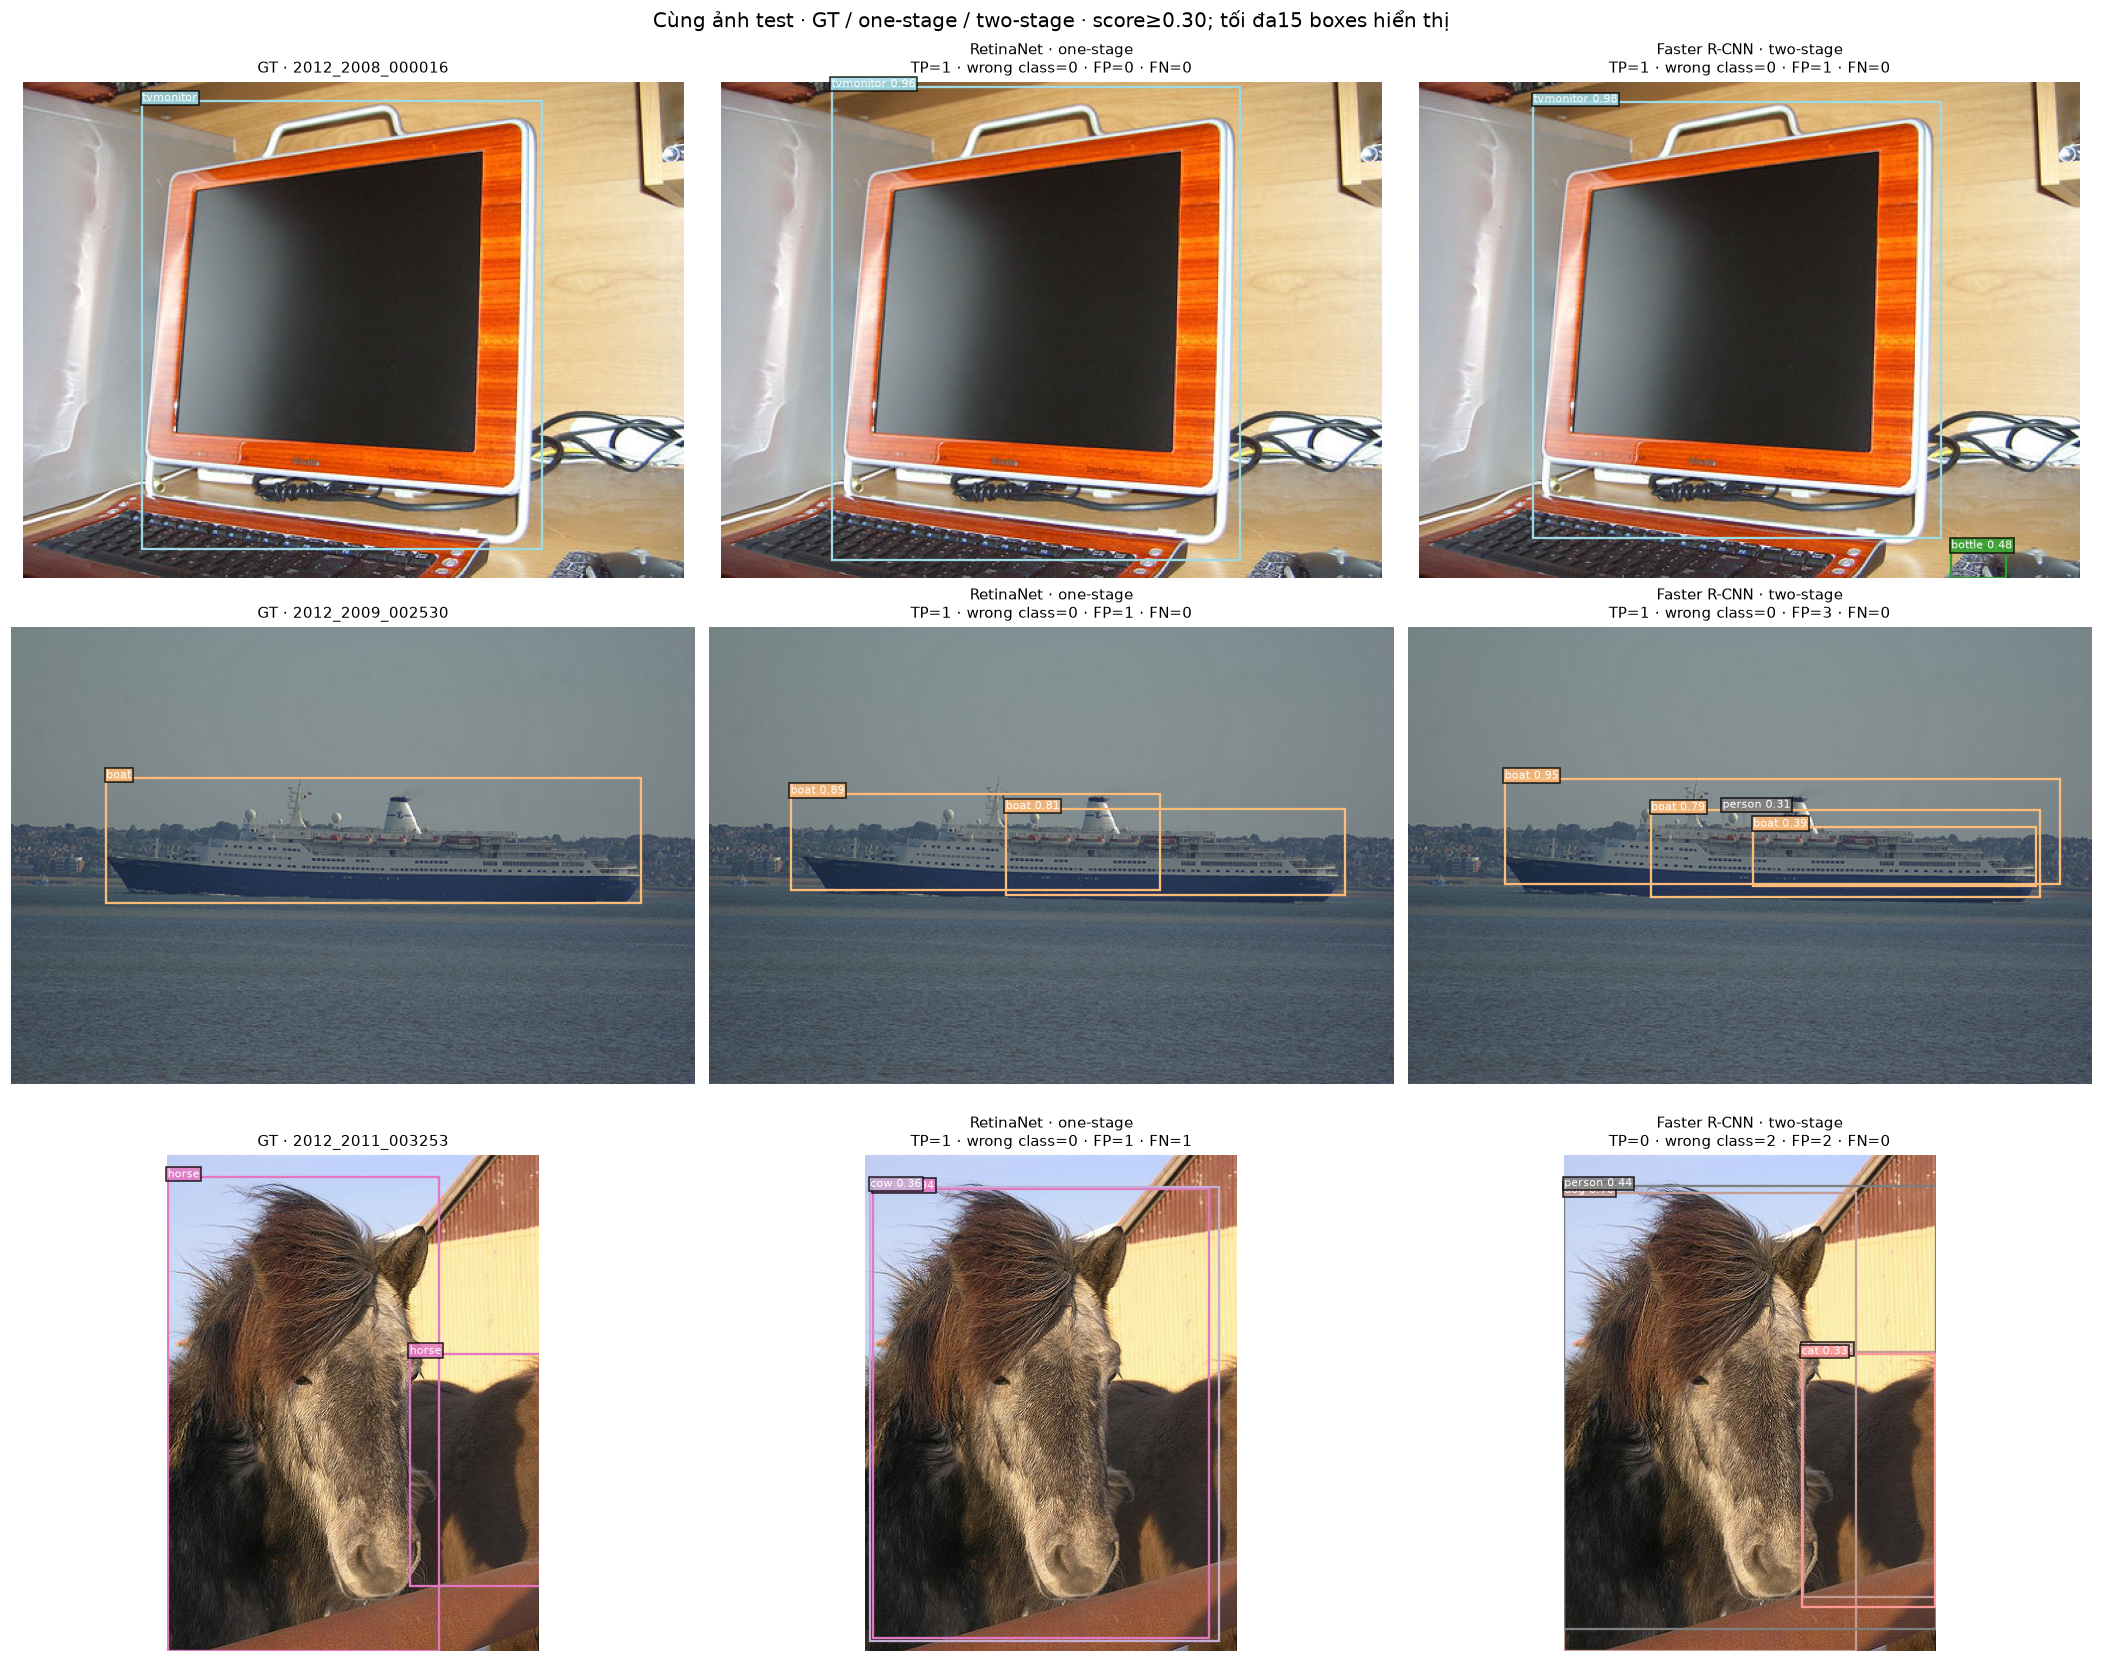
\includegraphics[width=.98\linewidth,height=.84\textheight,keepaspectratio]{assets/a2/predictions.png}
\caption{Cùng ba ảnh test: GT / RetinaNet / Faster R-CNN; score hiển thị 0,30, difficult nét đứt.}
\end{figure}\end{landscape}
\begin{landscape}\begin{figure}[p]\centering
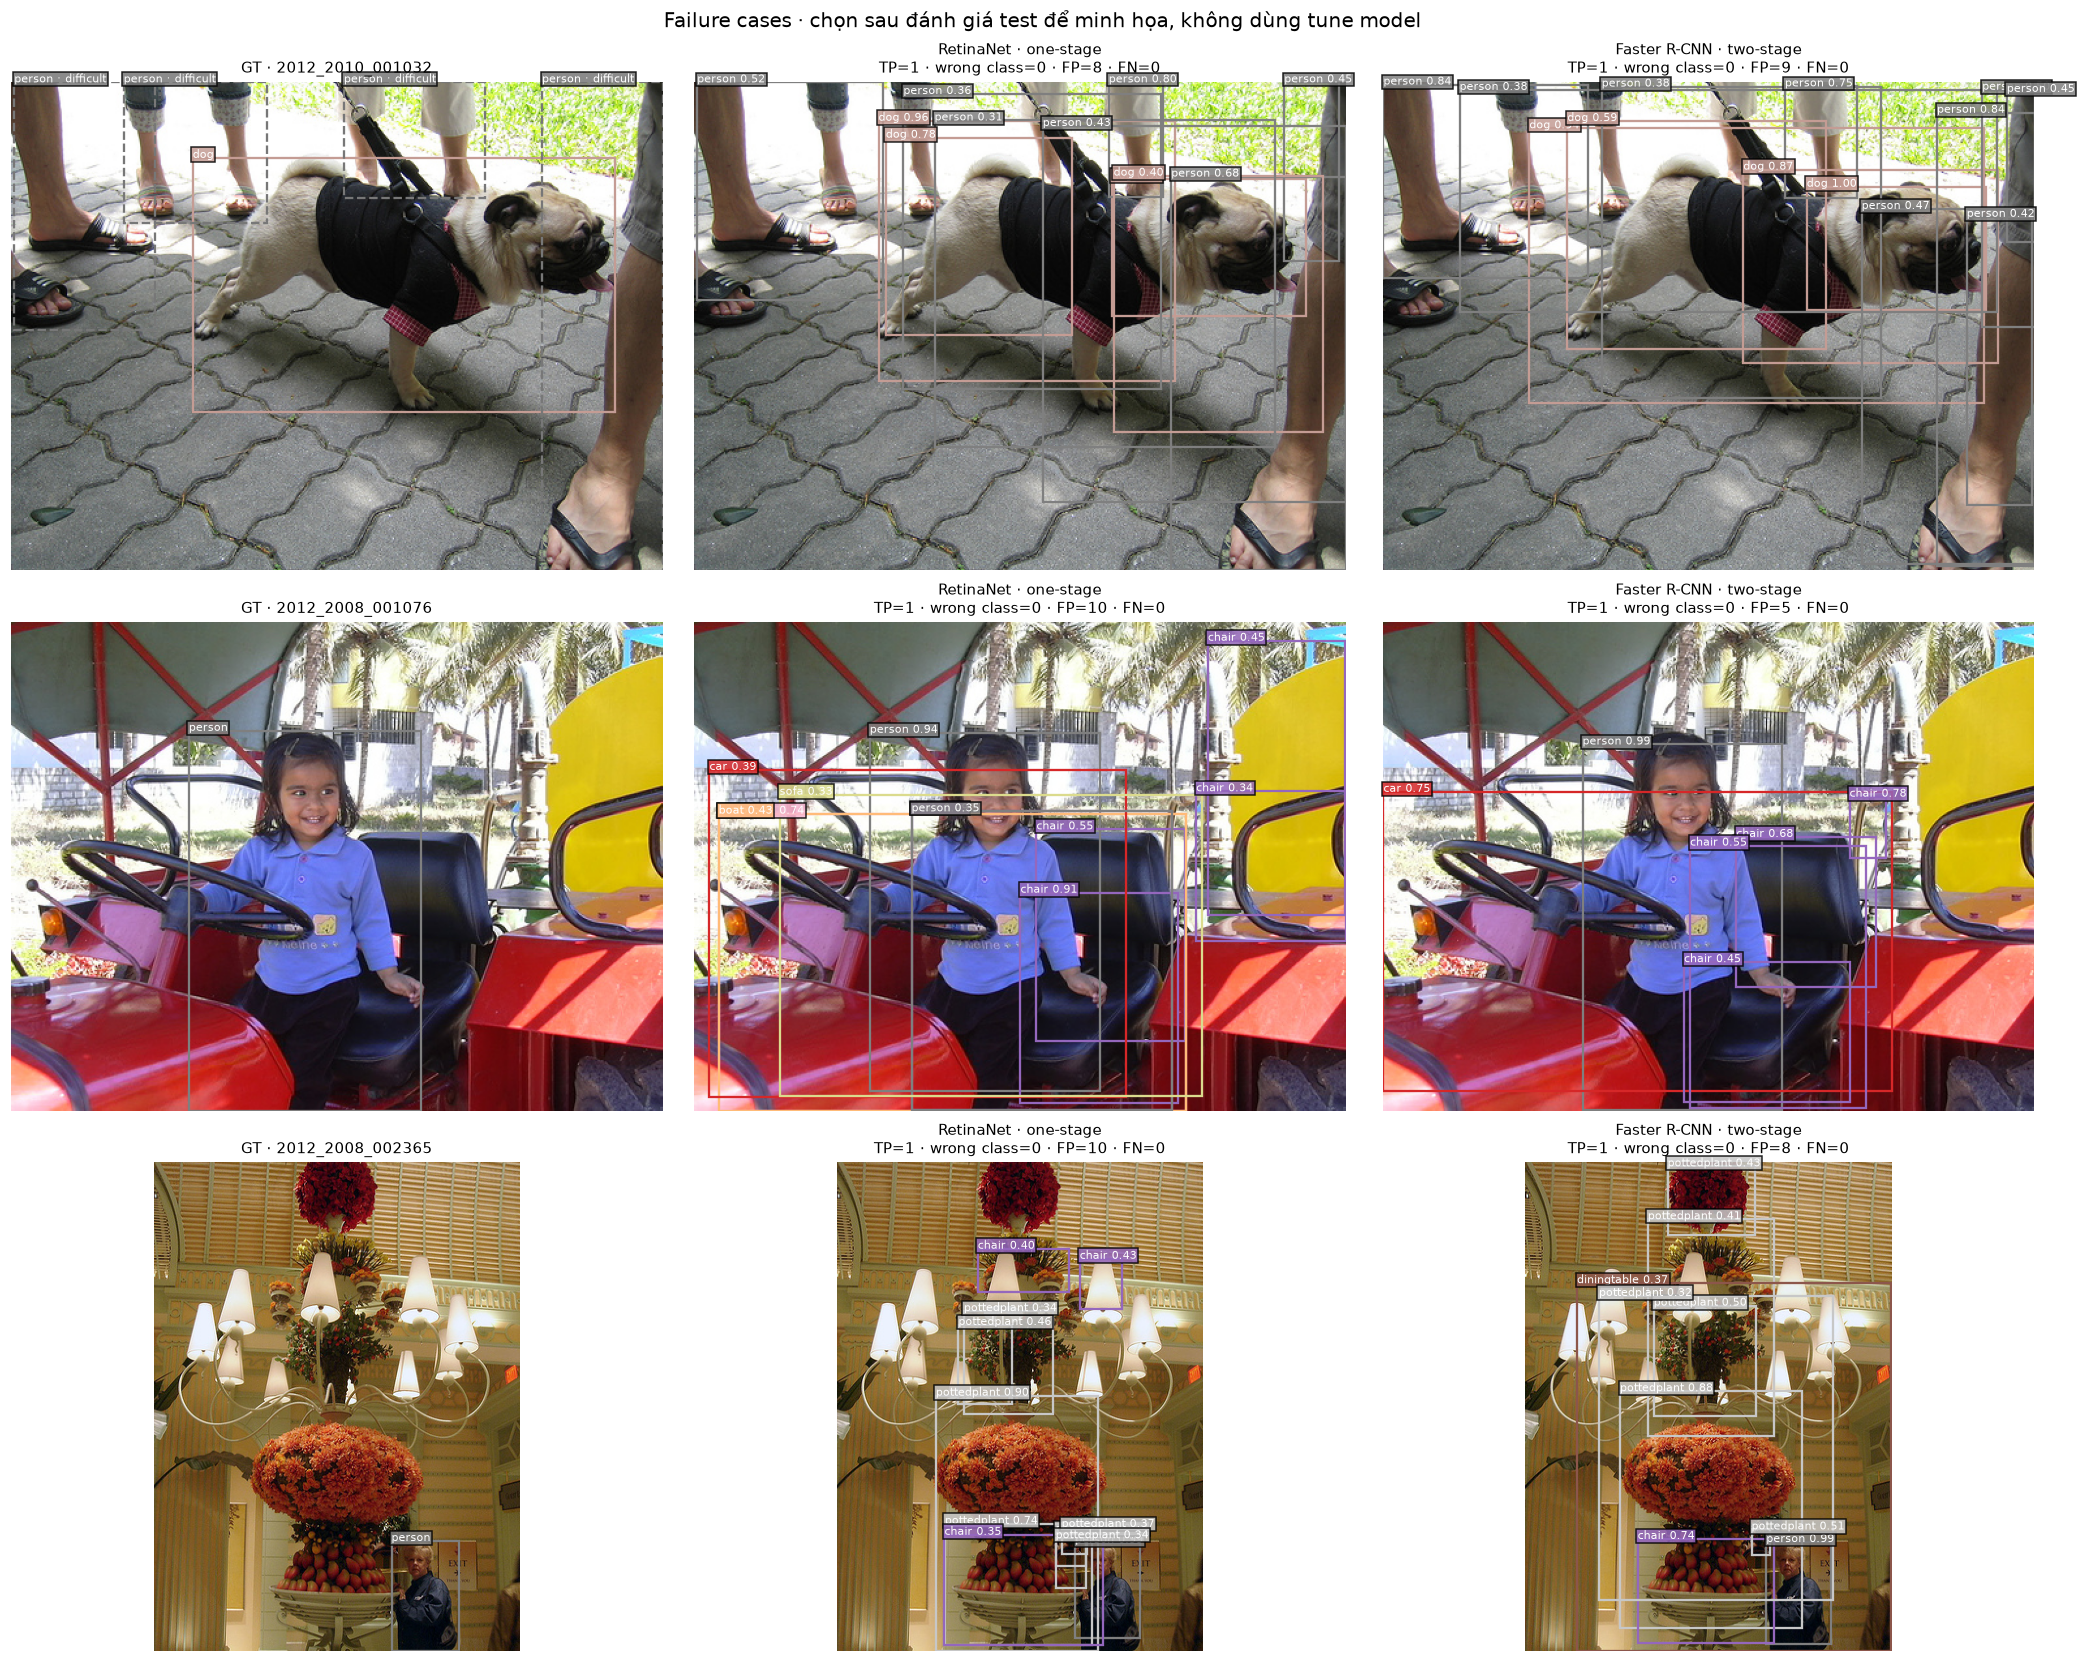
\includegraphics[width=.98\linewidth,height=.84\textheight,keepaspectratio]{assets/a2/failure_cases.png}
\caption{Ba ảnh có nhiều false positives: con chó, xe đồ chơi và trang trí nội thất. Các ví dụ được chọn sau test để phân tích, không dùng để chọn cấu hình.}
\end{figure}\end{landscape}
